% The document class supplies options to control rendering of some standard
% features in the result.  The goal is for uniform style, so some attention 
% to detail is *vital* with all fields.  Each field (i.e., text inside the
% curly braces below, so the MEng text inside {MEng} for instance) should 
% take into account the following:
%
% - author name       should be formatted as "FirstName LastName"
%   (not "Initial LastName" for example),
% - supervisor name   should be formatted as "Title FirstName LastName"
%   (where Title is "Dr." or "Prof." for example),
% - degree programme  should be "BSc", "MEng", "MSci", "MSc" or "PhD",
% - dissertation title should be correctly capitalised (plus you can have
%   an optional sub-title if appropriate, or leave this field blank),
% - dissertation type should be formatted as one of the following:
%   * for the MEng degree programme either "enterprise" or "research" to
%     reflect the stream,
%   * for the MSc  degree programme "$X/Y/Z$" for a project deemed to be
%     X%, Y% and Z% of type I, II and III.
% - year              should be formatted as a 4-digit year of submission
%   (so 2014 rather than the academic year, say 2013/14 say).

\documentclass[ % the name of the author
                    author={Ashrey Ashrey, Sanya Kapoor, Trisha Sharma, Yash Bhooshan Pandloskar},
                % the name of the supervisor
                supervisor={Dr. Dalila O’Grady},
                % the degree programme
                    degree={MSc},
                % the dissertation    title (which cannot be blank)
                     title={Using machine learning to forecast physical activity participation, volunteering and activity patterns in London},
                % the dissertation subtitle (which can    be blank)
                  subtitle={},
                % the dissertation     type
                      type={},
                % the year of submission
                      year={2021}]{dissertation}

\begin{document}

% =============================================================================

% This section simply introduces the structural guidelines.  It can clearly
% be deleted (or commented out) if you use the file as a template for your
% own dissertation: everything following it is in the correct order to use 
% as is.

\section*{Prelude}
\thispagestyle{empty}


A typical MSc thesis will be structured according to a fairly standard sequence of 
sections, and one example is shown here.  However, it is hard and perhaps even 
counter-productive to generalise: the goal of this document is {\em not}\/ to be prescriptive, to show you how you {\em must} structure your thesis; rather it is to simply to act as a guideline, to show you how you {\em could} structure your thesis.  In particular, each chapter's indicated page-count is
important but {\em not}\/ absolute: the aim is simply to highlight that a 
clear and concise description is better than a rambling alternative that makes
it hard to separate important content and facts from irrelevant trivia.

You can use this document as a \LaTeX-based 
template for your own thesis by simply deleting extraneous sections
and content, and adding your own text. If you do that, we recommend using BibTeX
to deal with the associated bibliography. 
You may want to use Overleaf (an online cloud-based collaborative \LaTeX platform).


The words ``thesis'' and ``dissertation'' are used interchangeably here. All active hyperlinks in the PDF file are rendered in the same shade of dark blue. 



% =============================================================================

% This macro creates the standard UoB title page by using information drawn
% from the document class (meaning it is vital you select the correct degree 
% title and so on).


\maketitle

% After the title page (which is a special case in that it is not numbered)
% comes the front matter or preliminaries; this macro signals the start of
% such content, meaning the pages are numbered with Roman numerals.

\frontmatter

% This macro creates the standard UoB declaration; on the printed hard-copy,
% this must be physically signed by the author in the space indicated.

\makedecl

% LaTeX automatically generates a table of contents, plus associated lists 
% of figures, tables and algorithms.  The former is a compulsory part of the
% dissertation, but if you do not require the latter they can be suppressed
% by simply commenting out the associated macro.

\tableofcontents
\listoffigures
\listoftables
\listofalgorithms
\lstlistoflistings

% The following sections are part of the front matter, but are not generated
% automatically by LaTeX; the use of \chapter* means they are not numbered.

% -----------------------------------------------------------------------------

\chapter*{Abstract} 
Physical inactivity remains an important public health challenge across London, where participation in sport, physical activity and volunteering varies considerably between boroughs and demographic groups, contributing to existing health inequalities. Although the Active Lives Survey provides extensive information on participation and its demographic correlates, existing research has largely focused on describing historical patterns rather than forecasting how participation may change in the future. This project develops a decision-support framework for producing borough-level forecasts of participation across London.
The project uses eight harmonised waves of the Active Lives Adult Survey from 2015–16 to 2022–23, covering respondents across all 32 London boroughs. The main challenge was the limited temporal information available for conventional forecasting. The dataset provides only 256 borough-year observations, with eight annual observations per borough and additional disruption associated with the COVID-19 pandemic. The project therefore separates the relationship between individual demographic characteristics and activity level from projected changes in population composition. An individual-level propensity model is combined with projected population characteristics to produce borough-level forecasts and distinguish changes associated with demographic composition from behavioural change.

\begin{quote}
Our research hypothesis is that separating a time-free demographic propensity model from a separately projected population will produce borough-level forecasts that are more statistically appropriate and interpretable for policy stakeholders than directly applying conventional forecasting models, without a substantial loss in predictive performance.
\end{quote}

\noindent
Main achievements:
\begin{quote}
\noindent
\begin{itemize}
\item Harmonised eight Active Lives Survey waves, resolving changes in variable definitions, category coding and borough identifiers. 
\item •	Developed an ordinal logistic regression propensity model and benchmarked it against LightGBM, achieving similar performance (AUC 0.704 and 0.707 respectively).
\item Developed a forecasting framework combining the propensity model with projected population characteristics to distinguish demographic composition effects from behavioural change.
\item Explored K-Modes with Random Forest, Bayesian hierarchical modelling and CatBoost with SHAP to inform and support the final methodology.
\item Produced borough-level outputs covering overall participation, demographic differences, the indoor–outdoor balance and volunteering as a decision-support resource.
\end{itemize}
\end{quote}
Overall, the findings support the proposed framework as a practical and interpretable alternative to directly applying conventional forecasting models to the limited borough-level time series available in the Active Lives data.

% -----------------------------------------------------------------------------

\chapter*{Summary of Changes}

{\bf A conditional section, of at most $1$ page} 
\vspace{1cm} 

If (and only if) the dissertation represents a resubmission (e.g., as the result of
a resit), then this section is compulsory: the content should summarise all
non-trivial changes made to the initial submission.  Otherwise you can
omit it, since {\bf a summary of this type is only needed for resubmissions}.

When included, the section will ideally be used to highlight additional
work completed, and address criticism raised in any associated feedback.
Clearly it is difficult to give generic advice about how to do so, but
an example might be as follows:

\begin{quote}
\noindent
\begin{itemize}
\item Feedback from the initial submission criticised the design and 
      implementation of my genetic algorithm, stating ``there seems 
      to have been no attention to computational complexity during the
      design, and obvious methods of optimisation are missing within
      the resulting implementation''.  Chapter 3 now includes a
      comprehensive analysis of the algorithm, in terms of both time
      and space.  While I have not altered the algorithm itself, I
      have included a cache mechanism (also detailed in Chapter 3)
      that provides a significant improvement in average run-time.
\item I added a feature in my implementation to allow automatic rather
      than manual selection of various parameters; the experimental
      results in Chapter 4 have been updated to reflect this.
\item Questions after the presentation highlighted a range of related
      work that I had not considered: I have make a number of updates 
      to Chapter 2, resolving this issue.
\end{itemize}
\end{quote}

% -----------------------------------------------------------------------------

\chapter*{Supporting Technologies}

{\bf A compulsory section, of at most $1$ page}
\vspace{1cm} 

\noindent
This section should present a detailed summary, in bullet point form, 
of any third-party resources (e.g., hardware and software components) 
used during the project.  Use of such resources is always perfectly 
acceptable: the goal of this section is simply to be clear about how
and where they are used, so that a clear assessment of your work can
result.  The content can focus on the project topic itself (rather,
for example, than including ``I used \mbox{\LaTeX} to prepare my 
dissertation''); an example is as follows:

\begin{quote}
\noindent
\begin{itemize}

\item I used the {\em Pandas} and {\em Seaborn} public-domian Python Libraries. 

\item I used a parts of the OpenCV computer vision library to capture 
      images from a camera, and for various standard operations (e.g., 
      threshold, edge detection).

\item I used Amazon Web Services for remote storage and processing of data. Specifically, I used:
 \begin{itemize}
 \item Simple Storage Service (S3) for data storage
 \item Elastic Compute Cloud (EC2) for provision of virtual machines
 \item Elastic Beanstalk for scaling and load management
 \item Sagemaker for all the machine learning components of my project. 
 \end{itemize}
 
\item I used \LaTeX\ to format my thesis, via the online service {\em Overleaf}. 
\end{itemize}
\end{quote}

% -----------------------------------------------------------------------------

\chapter*{Notation and Acronyms}

{\bf An optional section, of roughly $1$ or $2$ pages}
\vspace{1cm} 

\noindent
Any well written document will introduce notation and acronyms before
their use, {\em even if} they are standard in some way: this ensures 
any reader can understand the resulting self-contained content.  

Said introduction can exist within the dissertation itself, wherever 
that is appropriate.  For an acronym, this is typically achieved at 
the first point of use via ``Advanced Encryption Standard (AES)'' or 
similar, noting the capitalisation of relevant letters.  However, it 
can be useful to include an additional, dedicated list at the start 
of the dissertation; the advantage of doing so is that you cannot 
mistakenly use an acronym before defining it.  A limited example is 
as follows:

\begin{quote}
\noindent
\begin{tabular}{lcl}
AES                 &:     & Advanced Encryption Standard                                         \\
DES                 &:     & Data Encryption Standard                                             \\
                    &\vdots&                                                                      \\
${\mathcal H}( x )$ &:     & the Hamming weight of $x$                                            \\
${\mathbb  F}_q$    &:     & a finite field with $q$ elements                                     \\
$x_i$               &:     & the $i$-th bit of some binary sequence $x$, st. $x_i \in \{ 0, 1 \}$ \\
\end{tabular}
\end{quote}

% -----------------------------------------------------------------------------

\chapter*{Acknowledgements}

{\bf An optional section, of at most $1$ page}
\vspace{1cm} 

\noindent
It is common practice (although totally optional) to acknowledge any
third-party advice, contribution or influence you have found useful
during your work.  Examples include support from friends or family, 
the input of your Supervisor and/or Advisor, external organisations 
or persons who  have supplied resources of some kind (e.g., funding, 
advice or time), and so on.

\vspace{1cm}
Dave Cliff writes here to say huge thanks to his colleague Dr Dan Page for sharing this \LaTeX\ thesis template, which was originally written by Dan, for Computer Science dissertations. Dave edited Dan's original to better suit the needs of the Data Science MSc: please don't hassle Dan about any of this, but do feel free to contact Dave if you have any questions or comments on it.  

% =============================================================================

% After the front matter comes a number of chapters; under each chapter,
% sections, subsections and even subsubsections are permissible.  The
% pages in this part are numbered with Arabic numerals.  Note that:
%
% - A reference point can be marked using \label{XXX}, and then later
%   referred to via \ref{XXX}; for example Chapter\ref{chap:context}.
% - The chapters are presented here in one file; this can become hard
%   to manage.  An alternative is to save the content in seprate files
%   the use \input{XXX} to import it, which acts like the #include
%   directive in C.

\mainmatter

% -----------------------------------------------------------------------------

\chapter{Introduction}
\label{chap:introduction}

\section{Context and Problem Statement}
\noindent
Physical activity is one of the important factors that influences physical health, mental wellbeing and quality of life, though the level of participation varies significantly across various demographic groups and geographical areas, which contributes to chronic health inequalities and increased pressure on healthcare services.

London is an interesting city for researching participation due to the diverse population, socio-economic inequalities, and differences in access to sports facilities. Participation patterns vary across boroughs and different population segments, highlighting significant challenges in public health. These unequal levels of participation can contribute to wider health inequalities and also show that the benefits of being physically active are not distributed equally.

In order to effectively prepare for future changes, organisations and policymakers are eager to understand how this information can inform decisions regarding the allocation of resources and the implementation of health policies and drive impactful outcomes. General surveys of the country provide a large amount of information about historical participation and are primarily designed to describe what has happened rather than to predict what is likely to happen in the future.

This creates a practical problem for future participation: how can the available survey data be used to predict future participation when the data consist of repeated cross-sectional surveys rather than a panel of the same individuals over time? This predictive research problem is addressed by the current study, using data from 8 consecutive waves of the Active Lives Adult Survey (2015--16 to 2022--23), which includes data collected from participants in London that are spread across 32 London boroughs.

\section{Motivation and Contribution}

\noindent
The significance of this project can be considered from both a practical and a methodological perspective. From a practical perspective, borough-level forecasts of participation broken down by demographic group and activity type can provide the council or other organisations with evidence to support target-setting, resource allocation and the planning of interventions, as these forecasts will help in identifying those demographic groups and activities for which the forecasted change in participation is most important.

The project also addresses a gap in the limitations of the existing literature. The majority of studies based on the Active Lives Survey have mainly used regression or multilevel model analysis to explore the relationship between demographic factors and physical activity. However, not enough work has been done so far to predict future participation based on such a dataset. This is a complicated task because of the nature of this dataset, as it is repeated cross-sectional and its questionnaire structure and variable definitions have also changed across all the annual waves. Therefore, the project explores a forecasting approach which is suited to these characteristics of the data.

Conventional time-series or machine-learning forecasting methods cannot be applied directly to this problem because the amount of temporal data is limited. There are only eight annual survey waves, and the data is also affected by changes in the survey structure and the disruption caused by the COVID-19 pandemic. This project separates the relationship between individual characteristics and activity level from changes in the future population structure, instead of relying on a model to learn a complex time trend from these limited observations. The relationship between demographic characteristics and activity level is estimated using the full survey sample, which provides a large number of individual observations. Future population composition is projected separately and is used to estimate future participation. This approach also makes it possible to distinguish between changes caused by differences in demographic composition and changes in behaviour within demographic groups. This distinction is essential because an increase or decrease in overall participation may not necessarily mean that people's behaviour has changed, and it may partly result from changes in the characteristics of the population.

\section{Central Challenges}

\noindent
The design of the project is influenced by three main challenges, and these were the deciding factors for how the data should be analysed and how the forecasting approach should be developed.

\paragraph{Harmonising a survey that changes over time.} The Active Lives Survey is a repeated cross-sectional survey rather than a panel survey, which means that a new sample of respondents is collected in each annual wave. The structure of the survey also changed considerably across the eight waves used in this project. For example, the number of recorded variables increased from 292 to 601, while some variable definitions and local-authority identifiers changed between waves. The local-authority codes were affected by authority changes elsewhere in England, though the London boroughs themselves remained unchanged geographically. These differences needed to be resolved before the survey waves could be combined. Before the analytical stage, different members of the project team independently identified borough codes that had been incorrectly matched between waves. This highlighted the importance of carefully checking the geographic information before carrying out the later analysis, as such inconsistencies would silently corrupt every subsequent analytical stage.

\paragraph{Limited temporal information for conventional forecasting.} The dataset used contains 32 boroughs across eight annual waves, which gives 256 borough-year observations. Three of these waves were also affected by the disruption associated with the COVID-19 pandemic. This information is relatively limited for a time-series or machine-learning model to learn reliable temporal patterns. Instead of trying to learn a complex time trend from these few observations, the project therefore separates the relationship between demographic characteristics and activity from the projection of future population composition. This allows the larger individual-level survey sample to be used when estimating the demographic relationship, while population changes are considered separately when producing the forecasts.

\paragraph{Maintaining interpretability for a non-technical audience.} The forecasts are intended to support decision-making by local authorities and organisations around resource allocation and possible interventions. Therefore, interpretability was considered alongside predictive performance and computational efficiency. A more complex model is not necessarily more useful if its results are difficult for the intended audience to understand or justify. The final modelling approach was therefore selected based on a balance between predictive performance, interpretability and practical suitability.
This consideration is further discussed in Chapter~\ref{chap:background} and informed the comparison and selection of the final forecasting model.

\section{Summary of Aims, Objectives and Achievements}

\noindent
Based on the challenges discussed above, the overall aim and objectives of this project are as follows:

\noindent
\textbf{Aim:} To develop an interpretable borough-level forecasting framework for physical activity, sport and volunteering participation across London, using harmonised Active Lives Survey data from 2015--16 to 2022--23.

\begin{itemize}
\item \textbf{Objective 1:} To harmonise the eight Active Lives Survey waves into a consistent dataset by addressing inconsistencies in variable definitions, category coding and geographic coding.
\item \textbf{Objective 2:} To develop a propensity model that estimates the relationship between individual demographic characteristics and activity level, and to compare its performance with a more flexible gradient-boosting benchmark.
\item \textbf{Objective 3:} To investigate the extent to which the differences in participation between London boroughs can be explained by demographic composition and by borough-level differences.
\item \textbf{Objective 4:} To develop a forecasting approach that combines the propensity model with projected future population characteristics while distinguishing between changes that are associated with population composition and changes in behaviour.
\item \textbf{Objective 5:} To apply the framework to each of four areas: overall participation, demographic differences, the indoor--outdoor balance and volunteering. The results will then be presented in a form that can support decision-making by a non-technical stakeholder.
\end{itemize}

\noindent
These objectives provide a structured approach for the development and evaluation of the borough-level forecasting framework. The analysis also aims to provide a clearer understanding of the factors associated with differences in participation between London boroughs and how these differences may affect future forecasts.

% -----------------------------------------------------------------------------

\chapter{Background}
\label{chap:background}

\section{Problem Definition}

\noindent
Physical inactivity is one of the important and persistent public health challenges in London. Participation rates in sport and physical activity differ greatly between boroughs and different socio-economic groups, which could add to current health inequalities (Choe, Lee and Kang, 2025). The Active Lives Survey provides a comprehensive source of information for examining these differences. However, there are several characteristics of the survey that should be considered when it is used for forecasting. The survey is repeated cross-sectional, meaning that each annual wave contains a new sample of respondents rather than following the same individuals over time. In addition, the structure of the survey, variable definitions and category coding changed across the period covered by this project. Several of these changes were identified during the harmonisation of the 2015--16 to 2022--23 waves. For example, one socio-economic classification category was incorporated into an existing category from 2019--20 onwards. Similarly, the mid-level activity category was renamed from `Insufficiently Active' to `Fairly Active', although the underlying activity thresholds remained unchanged. These changes mean that these variables could not simply be combined across all waves without first evaluating whether their meanings were consistent.

Geographical identifiers provided another similar yet important issue. Local-authority codes are assigned across all English local authorities; if there is any change, such as mergers elsewhere in England, this can affect the numerical codes used for London boroughs in different survey waves. The London boroughs themselves have remained geographically fixed since 1965, but their numerical identifiers were not consistent across the survey files. Two members of the project team independently identified borough codes that had been incorrectly matched between waves using different verification procedures. This highlighted the potential for geographic coding errors to affect the analysis if they were not identified during the harmonisation stage. To address this issue, the local-authority codes from each wave were mapped using the relevant wave metadata to permanent Office for National Statistics Government Statistical Service identifiers. This provided a consistent geographic reference across the survey waves. These issues demonstrate that the forecasting problem cannot be considered solely in terms of selecting an appropriate modelling technique: the quality of the forecasting results also depends on whether the underlying survey data have been made sufficiently consistent across time. Careful harmonisation and validation were therefore treated as an important part of the modelling process rather than as a separate data-cleaning task.

\section{Domain Background: Determinants of Participation}

\noindent
Various studies have investigated the number of factors that might affect engagement in physical activities. The studies of Brainard et al. (2019), Brinkley et al. (2020) and Davis et al. (2011) have suggested that factors such as age, gender, socio-economic position, geography and neighbourhood are important determinants of participation. Similar trends have been identified in the current project, including age, socio-economic classification, disability and ethnicity, which were proved to be significant predictors of activity band. Research using the Active Lives Survey has mainly focused on describing and explaining existing trends of participation. Regression analyses and multi-level methods have been used to analyse the relationships between demographic factors and physical activity. They help to understand what factors are related to participation but do not suggest a way to estimate changes in the future. This difference between explaining existing patterns and forecasting future participation is important for the current project. Identification of the relationship between one demographic feature and physical activity does not necessarily mean that there is a way to make predictions about borough-level participation. The goal of the present research is to proceed from the existing knowledge of the factors affecting participation and use these relationships as part of a framework for estimating future participation at borough level.

\section{Forecasting Approaches Considered and Limitations of Conventional Models}

\noindent
Several modern machine-learning forecasting methods have been developed for structured temporal data. These include Gradient Boosting Machines (Chen and Guestrin, 2016; Ke et al., 2017), the Temporal Fusion Transformer (Lim et al., 2021) and N-BEATS (Oreshkin et al., 2020). These approaches have been successful in areas such as finance, energy, and health care. One possible approach in this case would be to estimate the activity rate per year for each of the boroughs, whether through data of borough per year or fitting a time series for each borough. However, the available data provides limited information for this type of approach. The dataset consists of 32 boroughs in 8 waves annually, which means that there are 256 borough-year observations. In addition, 3 of the waves include the disruption of the COVID-19 pandemic. Although each borough-year estimate is based on approximately 530 survey respondents, there are still only eight observations over time for each borough. This is challenging for the conventional time-series model to detect meaningful changes over time from variation in the survey estimates. Classical forecasting methods such as Prophet and ARIMA were also considered and were not selected for the borough-forecasting analysis for similar reasons. A weighted linear trend was instead used as a more conservative approach in a supplementary analysis. These results supported the decision not to make the borough forecasting component dependent on a complex temporal model.

The borough-forecasting model focuses on the relationship between demographic characteristics and activity level rather than attempting to learn a detailed borough-level time trend. The model is estimated to use the full sample to capture the relationship between individual characteristics and activity band. Future population characteristics are then projected separately and combined with the estimated model to produce borough-level forecasts. This approach also makes it possible for forecasted participation changes to be examined from two different angles. Certain changes may be due to variations in the demographic makeup of the group, whereas other changes might occur as a consequence of behavioural changes on the part of people who have the same demographics. This separation offers greater insight than just looking at a single overall time-series forecast and is useful when considering how future participation could be influenced through policy or interventions.

\section{The Borough-Forecasting Model}

\noindent
The outcome used in the borough-forecasting model is activity level, represented by three ordered categories: Inactive, Fairly Active and Active. As these activity levels can be categorised in an ordered manner, the ordered logit model was used which accounts for the ordering of the activities rather than assuming that they are independent of each other as in multinomial regression (McCullagh, 1980). The predictors included in the model were age band, gender, ethnicity, socio-economic classification, education, disability status, body-mass-index group and borough identity. Survey weights were also included during model fitting so that the estimates better reflect the population represented by the survey.

To finalise the main model, two different specifications were compared. Alongside the ordinal logistic regression, a gradient-boosting model using LightGBM (Ke et al., 2017) was also evaluated as a more flexible benchmark. The aim of this comparison was to check whether the introduction of a more complicated connection between predictors and activity level would result in some improvement in the prediction. The models were evaluated using a held-out survey wave. LightGBM achieved an AUC of 0.707, compared with 0.704 for the ordinal logistic regression. The difference in performance was small and was not practically meaningful. In addition to its similar predictive performance, it provides coefficients that can be interpreted directly and also makes the application of the model to future population characteristics easier. The comparison with LightGBM therefore provided the evidence that the additional complexity of a more flexible model did not provide a sufficient improvement in predictive performance to justify using it as the main model.

The model selection was also influenced by the limitations of the underlying data. Using a more complex algorithm does not remove the limitations created by having only eight annual survey waves and a repeated cross-sectional study design. The final model was therefore selected based on a combination of predictive performance, interpretability and suitability for the forecasting problem rather than predictive accuracy alone. The model was then used to generate individual-level activity predictions, which were then combined with projected future population characteristics to produce the borough-level forecasts presented in later chapters.

\section{Composition--Place Decomposition \& Model Interpretability}

\noindent
An important question to consider for the purpose of this research is the extent to which differences in activity across boroughs are due to individual characteristics of the people or to characteristics of the borough itself. This issue is significant for the forecasting process since projections for the future will take into account the change in demographic structure whereas characteristics of the place cannot be projected in the same way .To investigate this, three model specifications were compared: a demographics-only model, a borough-only model and a model including both demographic characteristics and borough identity. These models were compared based on how well they reproduced the observed variation in activity between boroughs. The demographics-only model was also evaluated using a leave-one-borough-out procedure, where each borough was predicted using a model trained without observations from that borough.

The demographics-only model explained 48\% of the variation between boroughs. When borough identity was included alongside the demographic variables, this increased to 88\%. This suggests that demographic composition accounts for a substantial part of the differences in participation between boroughs, while borough identity provides additional information. The leave-one-borough-out result was 47\%, which was very similar to the 48\% obtained from the corresponding demographics-only model. This provided evidence that the relationship between demographic characteristics and activity level is reasonably consistent across boroughs, including those that were not used to train the model. This is relevant to the forecasting approach because the model will be applied to projected population characteristics in the future. The composition-place method is connected with the demographic decomposition approach developed by Kitagawa (1955), where group differences are explained through differences in composition and differences in rates among the groups. This helps us to determine whether participation differences are due to the demographic make-up of the borough population or due to the borough itself.

Interpretability also plays a major role in choosing the primary method Molnar (2022). Both the ordinal regression and the composition-place analysis methods have interpretable coefficients that can be interpreted directly. For that reason, post-hoc interpretation tools such as SHAP (Lundberg and Lee, 2017) and variable importance using permutation (Fisher et al., 2019) were not applied to the primary model. Such methods are helpful, especially if the underlying model is not straightforward to interpret. SHAP was also applied separately in the gradient boosting analysis that was a part of the wider proje,ct which is discussed in Section 2.6. The results of the analysis serve as additional support for the conclusions rather than the primary method of interpreting the model.
\section{Alternative Approaches Explored}
\label{sec:alt-approaches}

\noindent
In addition to the borough-forecasting model described above, three alternative modelling approaches were undertaken as separate, independent workstreams within the wider project outlined in Chapter 3. Each approach addressed a distinct question in its own right and was developed and evaluated on its own terms. 

\paragraph{Demographic clustering and activity-level classification.} One approach combined unsupervised clustering of respondents based on demographic characteristics with supervised classification of overall activity level. K-Modes was used for the clustering because the main demographic variables, such as age band, gender and ethnicity, were categorical (Huang, 1997). Random Forest was then used to classify respondents according to their activity level (Breiman, 2001). This approach produced useful demographic segments and helped identify which characteristics were most informative for predicting activity level. However, since a CatBoost model was already being used as a separate approach for individual-level activity classification, this clustering-and-classification approach was found to be largely redundant. Its main contribution to the final methodology was the identification of demographic variables that were also considered in the propensity model.

\paragraph{Bayesian hierarchical modelling.} A second approach which was considered is the hierarchical structure of the survey data, with individuals nested within boroughs and boroughs within London. A Bayesian hierarchical model was developed with demographic characteristics as fixed effects and boroughs were included as a random effect by following the general Bayesian workflow Gelman et al. (2020) and the approach to grouped data discussed by Lunn et al. (2013). The models were fitted using Markov Chain Monte Carlo (MCMC) through PyMC/Stan. Individual model runs took approximately five to six hours, which limited the amount of iterations that could be carried out during the development. Despite this limitation, the analysis provided evidence that borough identity contains information beyond demographic composition. This finding was also examined through the composition–place analysis.

\paragraph{Gradient-boosted modelling, SHAP and borough residual analysis.} A third workstream used a CatBoost gradient-boosting classifier for the individual-level prediction task. The model was trained on waves one to seven and evaluated on the final wave. This temporal validation approach was preferred over a random train-test split because it reduces the risk of using information from a later wave when predicting an earlier stage of the analysis. The model achieved an AUC score of 0.708, which was very similar to the performance obtained from the models considered in the primary pipeline. SHAP analysis (Lundberg and Lee, 2017) was used to investigate the importance of the predictors. Age was the most influential variable, which was followed by ethnicity, education and social grade. Using this pipeline, we also examined borough-level residuals using a leave-one-wave-out procedure. Nine boroughs showed a stable, sign-consistent effect across at least seven of the eight waves. This effect remained when controlling for area deprivation, with a correlation of −0.06. These results provided additional evidence that differences between boroughs may not be explained entirely by demographic composition.

An additional borough-level forecast was also developed using a weighted linear trend. This approach was chosen after some time-series methods (Prophet, ARIMA), which are more flexible but were considered unsuitable due to the short length of only eight annual years. Another separate activity-type analysis examined the contribution of individual activities to the 150-minute weekly activity threshold and showed that walking and active travel were responsible for a significant part of the activity rate of Londoners. However, numerous valuable insights were gained through this approach; it was not chosen as the primary forecasting method as it did not provide any distinguish between demographic composition and behavioural change and SHAP analysis gave data which could be easily obtained via interpretable coefficients of ordinal regression. Although, borough residual and activity-level analysis were helpful in corroborating insights gained from the main method of forecasting.

\section{Related Work and Research Gap}

\noindent
Another study employed various machine learning techniques to predict adherence to physical activity guidelines based on data collected from cross-sectional surveys (Choe, Lee and Kang, 2025). Six algorithms were tested, and the results revealed that features such as sedentary behaviour, age, gender and education were most useful for prediction. This shows that machine learning techniques could be applied to predict physical activity outcomes at an individual level. However, that study focuses on current adherence rather than changes in the future and does not provide geographically disaggregated forecasts. The literature and methodological considerations reviewed in this chapter reveal four gaps that the present project addresses.

\begin{enumerate}
\item While repeated cross-sectional surveys can provide a large number of individual observations, they may contain changes in questionnaire structure, variable definitions and coding between waves. Additional challenges can arise when the data is used for forecasting rather than simply describing historical patterns.
\item An application gap exists in existing research using the Active Lives Survey. Most studies have mainly focused on describing levels of participation or investigating relationships between demographic characteristics and activity, and fewer attempts have been made to use the survey to produce future participation forecasts.
\item Methods such as Gradient Boosting Machines, the Temporal Fusion Transformer and N-BEATS can be effective when sufficient temporal data is available. However, the Active Lives data contain only eight annual waves at borough level, which means that a complicated forecasting model cannot learn reliable temporal patterns specific to each borough. Instead, the method proposed in this project leverages the existing individual-level data to estimate a time-free relationship between demographic characteristics and activity, and then combines this with future population projections.
\item There is limited literature that combines harmonised multi-year Active Lives data with borough-level forecasting while considering the possibility of future changes due to demographic differences or behavioural change. This is an important gap to address because a change in participation does not necessarily imply a change in the behavioural pattern of the borough, as it may result from changes in the population structure of a borough.
\end{enumerate}

\noindent
These gaps motivate the methodology described in subsequent chapters. The project begins with the harmonisation of the survey data, followed by the development and validation of the propensity model, examines the association between demographics and borough, and uses these components within the forecasting framework.

% -----------------------------------------------------------------------------

\chapter{Methodology}
\label{chap:methodology}

\section{Overall Project Workflow}

\noindent
This project followed a structured five-stage machine learning pipeline, transforming raw Active Lives Survey data into borough-level forecasts across four analytical pillars: \emph{P1} overall physical activity participation, \emph{P2} demographic-specific participation, \emph{P3} indoor versus outdoor activity, and \emph{P4} sport volunteering. The workflow was designed to ensure that data quality issues were addressed before modelling, enabling the development of reliable, interpretable and generalisable predictive models.

\begin{description}
\item[Stage 1 -- Data Preparation and Harmonisation:] Eight structurally inconsistent annual survey files were merged into a single individual-level dataset. Preprocessing was required to standardise variable names, harmonise borough identifiers using permanent ONS GSS codes, resolve inconsistencies in Local Authority coding, and handle sentinel/missing values.
\item[Stage 2 -- Exploratory Data Analysis:] a quality-assurance EDA targeting six specific risk areas associated with a multi-wave government survey: merge integrity, sentinel contamination, missingness, borough coverage, cross-year consistency and distributional plausibility.
\item[Stage 3 -- Feature Engineering:] the cleaned master dataset, containing 610 variables, was reduced to a compact model-ready dataset, with the ordinal \texttt{Activity\_Level} target derived and demographic predictors consolidated.
\item[Stage 4 -- Machine Learning Modelling:] Four complementary modelling approaches were developed in parallel to address different components of the problem: an individual-level driver model (CatBoost with SHAP), a borough-forecasting propensity model (ordinal logistic regression benchmarked against LightGBM), a demographic segmentation and prediction pipeline (K-Modes clustering with supervised classifiers), and a fully probabilistic borough random-effects model (Bayesian Hierarchical Ordinal Logistic Regression).
\item[Stage 5 -- Forecasting and Scenario Analysis:] combines the outputs of the predictive models to generate borough- and London-level forecasts. Forecasts are produced by integrating estimated participation propensities with projected demographic compositions and behavioural trends, allowing overall changes to be decomposed into demographic composition effects and behavioural effects. Activity-type perturbation decomposes the aggregate active rate by the nine Sport England activity-method groups, isolating each activity's marginal contribution to the 150-minute threshold by removing its minutes and re-testing participation. Walking is found to be the dominant load-bearing activity at London level, while a borough-level comparison shows over-performing boroughs leaning more on cycling and adventure/water sports, and under-performing boroughs relying more heavily on walking alone -- an indicative, infrastructure-linked signature rather than a causal claim.
\end{description}

\noindent
The overall workflow connecting these five stages is summarised in Figure~\ref{fig:workflow}.

\begin{figure}[t]
\centering
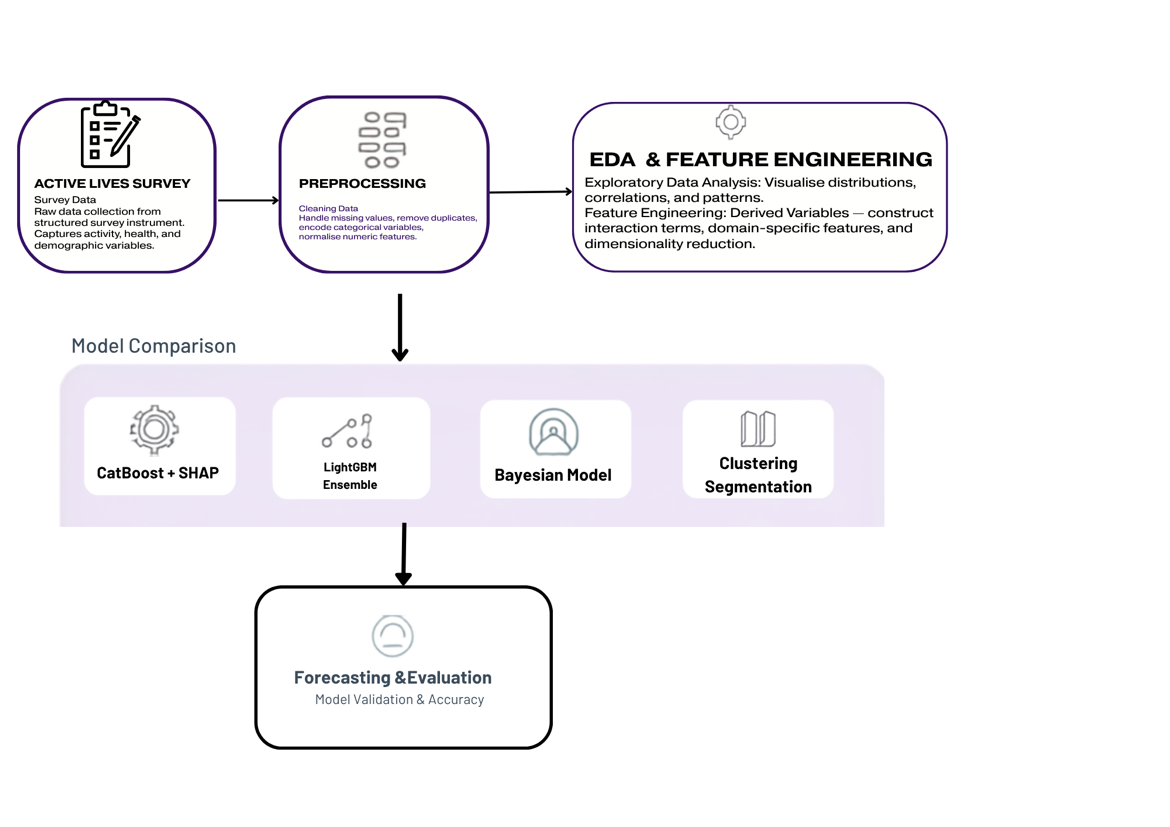
\includegraphics[width=0.7\textwidth]{figures/fig3_1_workflow}
\caption{Overall project workflow diagram.}
\label{fig:workflow}
\end{figure}

\noindent
A consistent validation principle was applied across all four modelling strands: rather than using random train--test splits, a time-based validation framework was used. Models were trained using the first seven years of data and tested on the final 2022--23 survey wave. This approach closely reflects the real-world forecasting problem by ensuring that predictions are generated using only historical information, thereby preventing information leakage and providing a more realistic assessment of model generalisation.

\section{Dataset Description}

\noindent
The analysis uses data from Sport England's Active Lives Adult Survey, a nationally representative survey that measures physical activity participation among adults aged 16 years and above in England. The survey collects information on physical activity behaviour, demographic characteristics, health, education, volunteering and other lifestyle factors using a repeated cross-sectional design. Unlike a longitudinal study, respondents are not followed over multiple years; instead, a new sample is collected annually.

Eight consecutive survey waves, spanning 2015--16 to 2022--23, were used. After filtering the national dataset to Greater London and excluding the City of London, the final dataset comprised 135,497 respondents across 32 London boroughs. Although each raw survey contained approximately 10,700 variables, only variables relevant to the four analytical pillars were retained. As additional question blocks were introduced in later survey waves, the number of columns increased from 292 in the first wave to 601 in the final wave. Table~\ref{tab:dataset-summary} summarises the key properties of the dataset.

\begin{table}[t]
\centering
\caption{Dataset summary.}
\label{tab:dataset-summary}
\begin{tabular}{|l|l|}
\hline
\textbf{Property} & \textbf{Value} \\
\hline
Data source              & Sport England Active Lives Adult Survey (UKDS Ref. 9288) \\
Survey period             & 2015--16 to 2022--23 \\
Survey waves              & 8 \\
Study area                & 32 London boroughs \\
Total respondents         & 135,497 \\
Raw variables (per wave)  & $\sim$10,700 \\
Merged dataset variables  & 610 \\
\hline
\end{tabular}
\end{table}

\section{Data Preprocessing}

\noindent
Before model development, a single consistent analytical dataset was required. The Active Lives Survey evolved over time, with different geographical coding, variable availability, naming conventions and survey structure. During preprocessing, the focus was on harmonising inconsistencies while preserving the integrity of the original survey data. The overall preprocessing workflow is illustrated in Figure~\ref{fig:preprocessing}.

\begin{figure}[t]
\centering
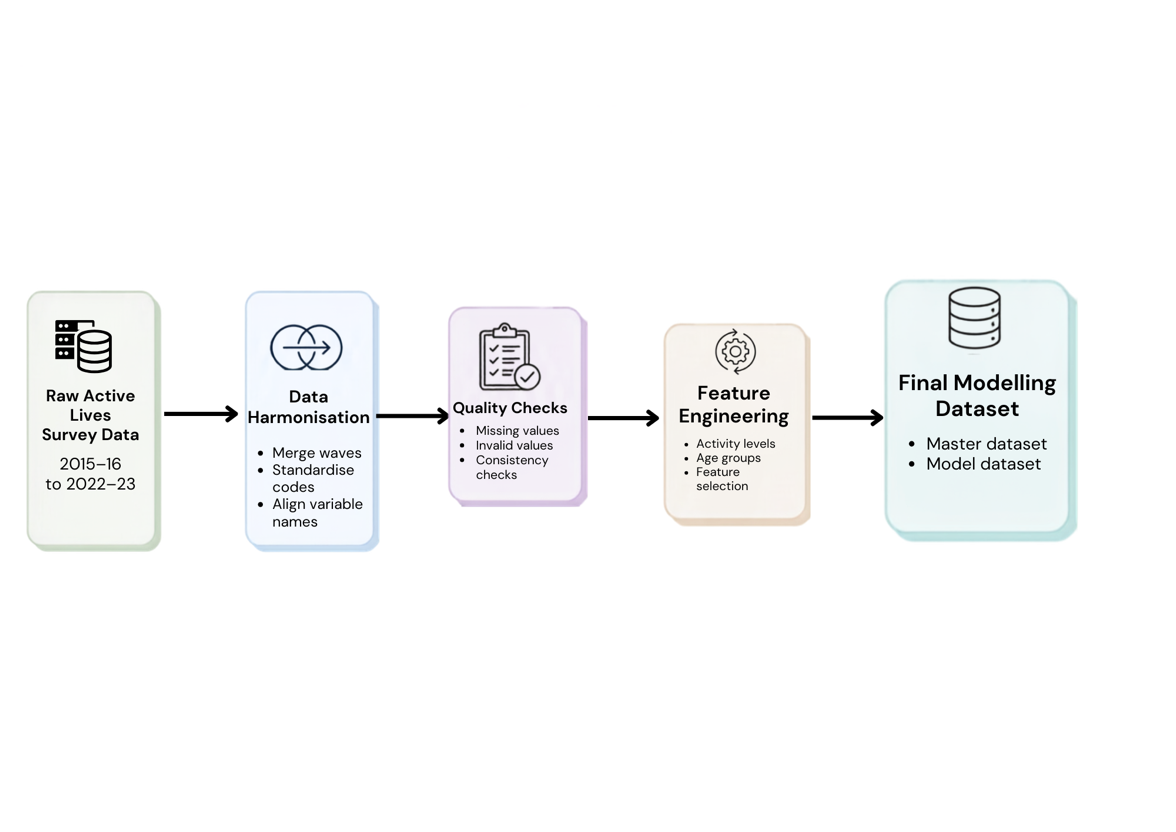
\includegraphics[width=0.6\textwidth]{figures/fig3_2_preprocessing}
\caption{Data preprocessing workflow showing dataset harmonisation, data quality checks, feature engineering, and creation of the final modelling datasets.}
\label{fig:preprocessing}
\end{figure}

\subsection{Data Harmonisation}

\noindent
The first stage was harmonising the eight survey waves into a unified dataset. Borough identities were standardised using the permanent \textbf{ONS Government Statistical Service (GSS)} codes to ensure that each London borough remained consistently identified across all survey years. Variable names were also standardised where naming conventions had changed between survey waves, to merge equivalent variables into a common schema. These steps ensured that the final merged dataset contained consistent geographical and variable identifiers across the entire study period.

\subsection{Missing Data and Data Quality}

\noindent
Data quality checks were performed to identify missing values, invalid entries and inconsistencies across survey waves. During import, it was essential to convert the SPSS sentinel values representing non-response into missing values, to prevent invalid numeric codes from influencing the prediction. The remaining missing values arose primarily from survey routing or from questions introduced in later survey waves, rather than from data corruption.

Rather than imputing missing values, the original survey structure was preserved wherever possible. Some variables, such as health, were unavailable in earlier survey years and remained missing for those years. Optional demographic non-response categories were retained as explicit categories to avoid unnecessary information loss. Minor inconsistencies in categorical labels across survey years were standardised to ensure a consistent coding framework throughout the merged dataset.

\subsection{Feature Engineering}

\noindent
Feature engineering transformed the harmonised dataset into a model-ready format. The primary target variable, \texttt{Activity\_Level}, was derived from the variable \texttt{MEMS7\_ALL} (number of minutes of moderate-intensity activity per week): Inactive (0--29 minutes/week), Fairly Active (30--149 minutes/week), and Active (150 or more minutes/week). The resulting target variable was stored as an ordered categorical variable to preserve its ordinal structure for modelling. The resulting distribution of the target variable is shown in Table~\ref{tab:activity-level}.

\begin{table}[t]
\centering
\caption{Distribution of the derived \texttt{Activity\_Level} target variable.}
\label{tab:activity-level}
\begin{tabular}{|l|l|r|r|}
\hline
\textbf{Activity Level} & \textbf{\texttt{MEMS7\_ALL} Threshold} & \textbf{Count} & \textbf{\% of Dataset} \\
\hline
Active         & 150+ minutes/week      & 90,124 & 66.5\% \\
Fairly Active  & 30--149 minutes/week   & 15,033 & 11.1\% \\
Inactive       & 0--29 minutes/week     & 30,340 & 22.4\% \\
\hline
\end{tabular}
\end{table}

\noindent
To improve interpretability and maintain adequate sample sizes, the age variable, originally recorded using nine age categories, was redefined into four broad age groups (16--24, 25--44, 45--64 and 65+), as detailed in Table~\ref{tab:age-groups}. All categorical predictors were converted to categorical data types to improve computational efficiency and ensure compatibility with the machine learning algorithms.

\begin{table}[t]
\centering
\caption{Construction of the four broad age groups from the original nine-band age variable.}
\label{tab:age-groups}
\begin{tabular}{|l|l|r|}
\hline
\textbf{Age\_Group} & \textbf{Age9 Bands Included} & \textbf{Count} \\
\hline
16--24 & 16--24                 & 11,110 \\
25--44 & 25--34, 35--44         & 53,216 \\
45--64 & 45--54, 55--64         & 43,555 \\
65+    & 65--74, 75--84, 85+    & 26,289 \\
\hline
\end{tabular}
\end{table}

\subsection{Final Modelling Dataset}

\noindent
The final master dataset contained 135,497 respondents and 610 variables. To improve modelling efficiency, two purpose-specific datasets were created. For the CatBoost, clustering and Bayesian models, a compact 20-variable dataset (containing demographic characteristics, activity measures and the derived target variable) was used. For activity-type information, a broader dataset with approximately 75 variables was used in the LightGBM model. Additionally, borough-level aggregated datasets were created to support trend analysis and borough-level forecasting, although these were not used for model training.

\section{Exploratory Data Analysis}

\noindent
Exploratory Data Analysis (EDA) was conducted after preprocessing to understand the characteristics of the harmonised dataset and identify patterns that could influence model development. The EDA was carried out in two stages. First, each survey wave was analysed individually to examine borough coverage, demographic distributions and data completeness before merging. The second stage was a weighted EDA conducted on the harmonised single dataset, to explore London-wide demographic, geographical and temporal patterns. This approach ensured that any wave-specific inconsistencies were identified before they could influence the merged dataset.

The weighted exploratory analysis had four key objectives: respondents' demographic characteristics, trends in physical activity by year, geographical variation across boroughs, and volunteering behaviour. These analyses provided a better understanding of the study population, helped identify important patterns in the data, and informed the feature selection and modelling approaches used in the later stages of the project.

\subsection{Population Characteristics}

\noindent
The demographic characteristics of the study population were explored using population-weighted summaries of age, gender, ethnicity, education and disability status, as shown in Figure~\ref{fig:demographics}. Examining these distributions helped establish an overall profile of the London population represented in the survey, and showed clear differences across demographic groups, supporting their use as important predictor variables in the subsequent modelling.

\begin{figure}[t]
\centering
\begin{minipage}{0.48\textwidth}
\centering
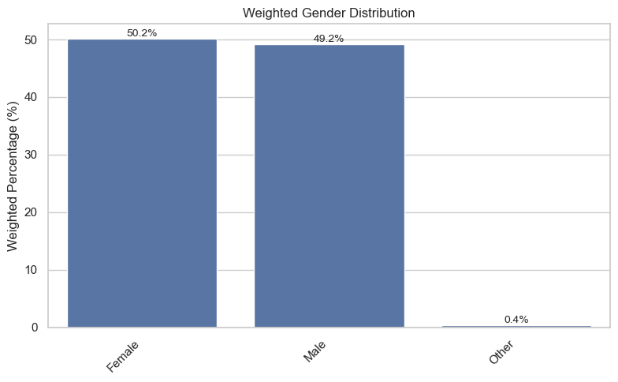
\includegraphics[width=\textwidth]{figures/fig3_3a_demographics}
\end{minipage}\hfill
\begin{minipage}{0.48\textwidth}
\centering
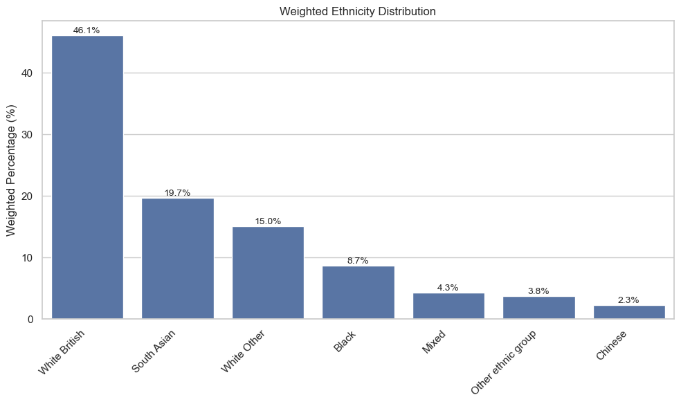
\includegraphics[width=\textwidth]{figures/fig3_3b_demographics}
\end{minipage}

\vspace{0.5cm}

\begin{minipage}{0.32\textwidth}
\centering
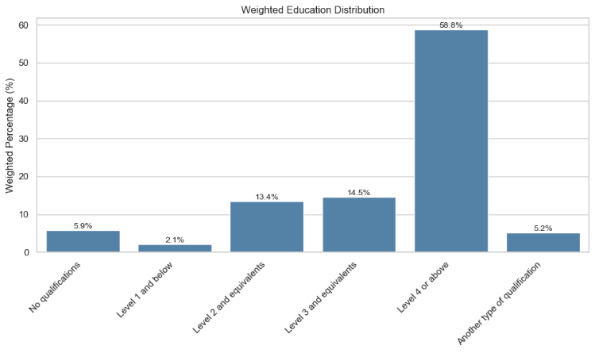
\includegraphics[width=\textwidth]{figures/fig3_3c_demographics}
\end{minipage}\hfill
\begin{minipage}{0.32\textwidth}
\centering
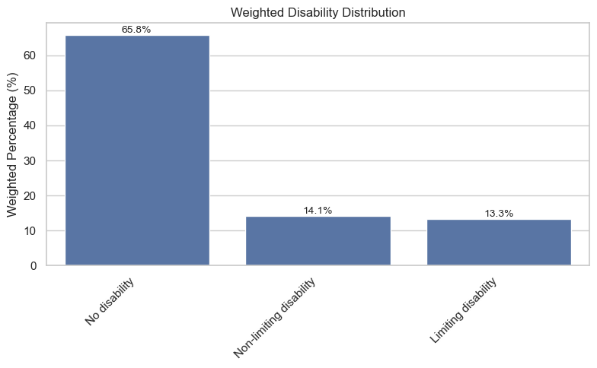
\includegraphics[width=\textwidth]{figures/fig3_3d_demographics}
\end{minipage}\hfill
\begin{minipage}{0.32\textwidth}
\centering
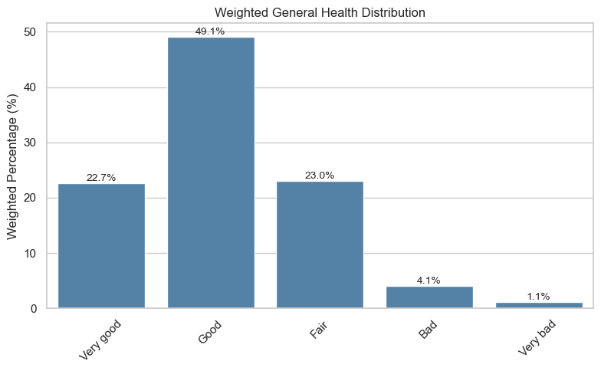
\includegraphics[width=\textwidth]{figures/fig3_3e_demographics}
\end{minipage}
\caption{Population-weighted demographic characteristics of respondents.}
\label{fig:demographics}
\end{figure}

\subsection{Physical Activity Trends}

\noindent
Physical activity levels were analysed across all eight survey waves using the derived \texttt{Activity\_Level} variable, as shown in Figure~\ref{fig:activity-trends}. Throughout the study period, overall participation was stable; however, there was a temporary spike in inactivity during the COVID-19 pandemic, followed by a gradual recovery in later years. The proportion of respondents classified as Fairly Active also showed a gradual decline in later years, suggesting changes in participation behaviour over time.

Spatial analysis, shown in Figure~\ref{fig:borough-variation}, further demonstrated that activity levels varied across London's boroughs, indicating that geographical location may influence physical activity participation. These observations supported the inclusion of borough-level effects within the forecasting and Bayesian modelling frameworks.

\begin{figure}[t]
\centering
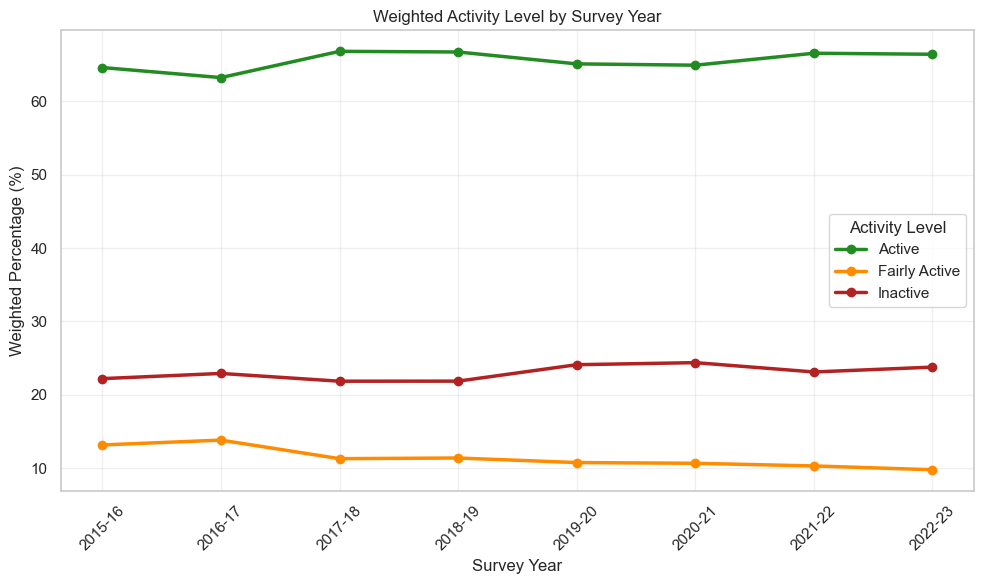
\includegraphics[width=0.75\textwidth]{figures/fig3_4_activity_trends}
\caption{Population-weighted distribution of activity levels across survey years.}
\label{fig:activity-trends}
\end{figure}

\begin{figure}[t]
\centering
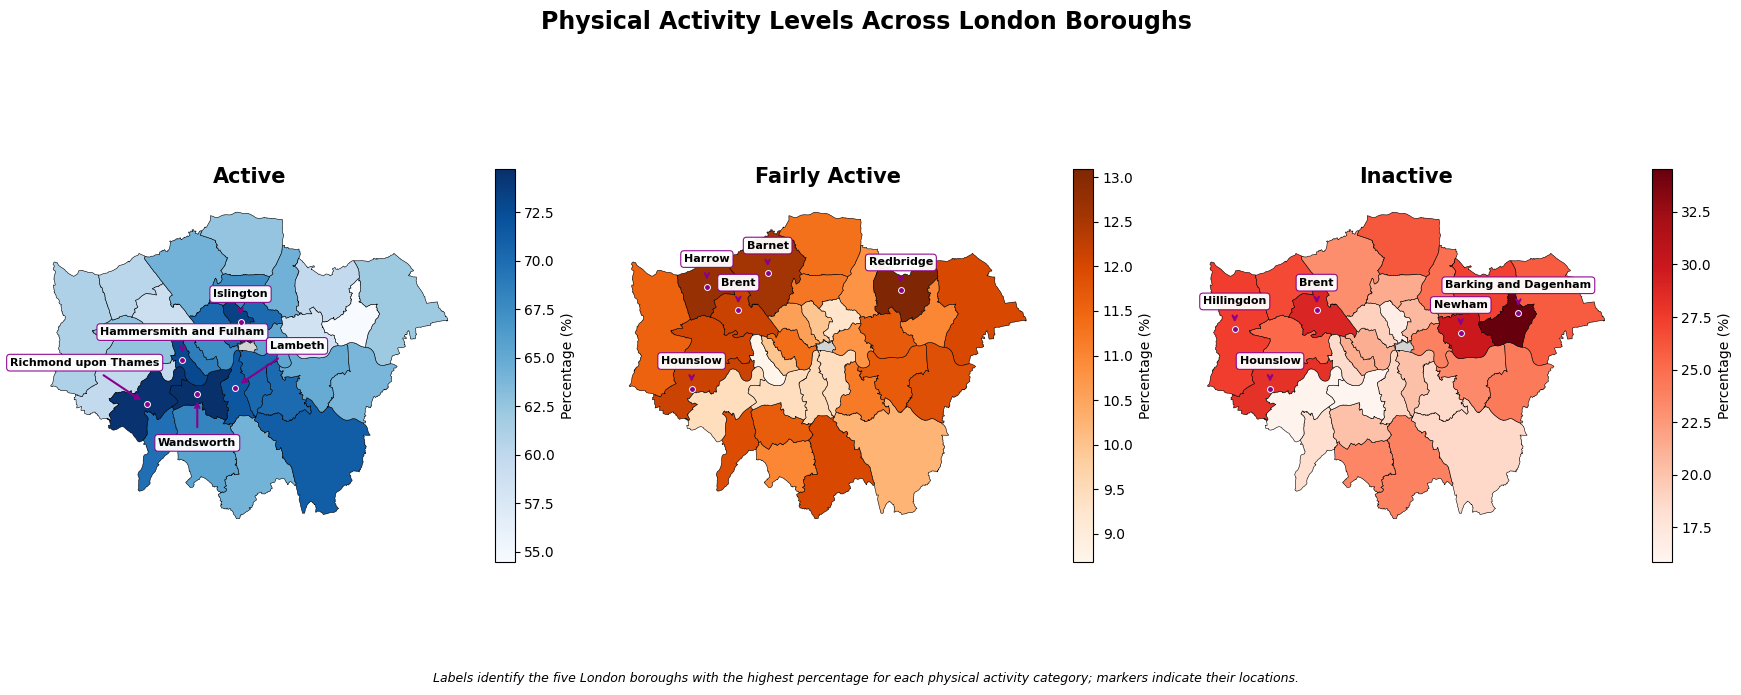
\includegraphics[width=\textwidth]{figures/fig3_5_borough_variation}
\caption{Geographical variation in population-weighted activity levels across London's boroughs.}
\label{fig:borough-variation}
\end{figure}

\subsection{Volunteering Trends}

\noindent
Volunteering was analysed to understand how participation changed over time, as shown in Figure~\ref{fig:volunteering}. The results showed that volunteering levels fell during the COVID-19 period before gradually recovering in the following survey years. A noticeable change between the 2017--18 and 2018--19 survey waves was also observed, which aligns with revisions made to the Active Lives Survey rather than reflecting a genuine change in volunteering behaviour. Identifying these patterns helped provide context for the forecasting analysis presented in later chapters.

\begin{figure}[t]
\centering
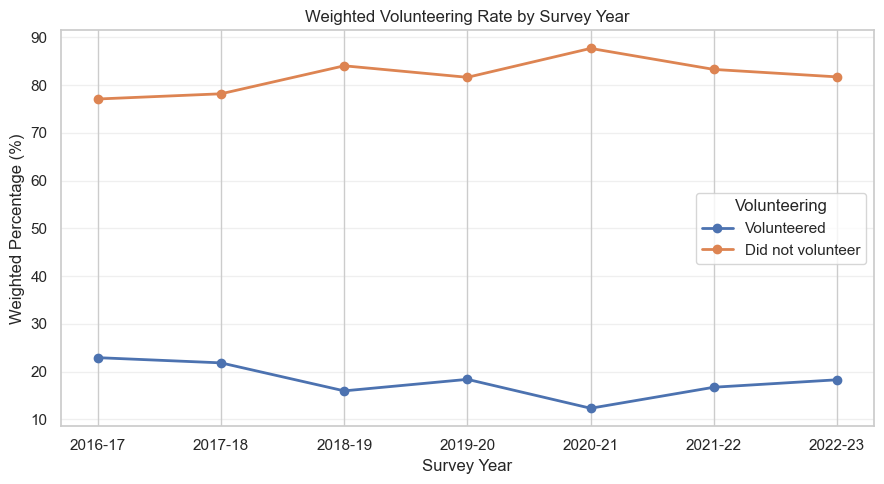
\includegraphics[width=0.75\textwidth]{figures/fig3_6_volunteering}
\caption{Population-weighted volunteering participation across survey years.}
\label{fig:volunteering}
\end{figure}

\section{Machine Learning Framework}

\noindent
To address the objectives of the London Sport project, four different machine learning approaches were developed and evaluated independently. Rather than relying on a single model, multiple techniques were explored because each model offers different strengths in analysing physical activity data. Some models are better suited to prediction, others provide greater interpretability or uncertainty estimation, while some are useful for identifying hidden patterns within the population. Using a range of approaches also allowed their performance to be compared under the same data and validation framework before selecting the most suitable models for forecasting and interpretation.

The four modelling approaches included \textbf{CatBoost with SHAP}, \textbf{LightGBM}, \textbf{K-Modes clustering}, and a \textbf{Bayesian Hierarchical Ordinal Logistic Regression} model. CatBoost was selected for its strong performance on structured datasets containing many categorical variables, while SHAP was used to explain the contribution of each predictor to the model's decisions. LightGBM was chosen as an alternative gradient-boosting approach because of its computational efficiency and ability to handle high-dimensional tabular data. K-Modes clustering was applied to identify groups of respondents with similar demographic and participation characteristics, giving additional insight into population segmentation. Finally, the Bayesian hierarchical model was developed to account for the ordered nature of the activity outcome while capturing variation between London boroughs through random effects and providing probabilistic estimates of uncertainty.

To ensure a fair comparison, all four models were developed using the same modelling dataset and evaluated under the same validation strategy. Survey data from \textbf{2015--16 to 2021--22} were used for model development, while the final \textbf{2022--23} survey wave was used as an unseen test dataset.

% -----------------------------------------------------------------------------

\chapter{Critical Evaluation}
\label{chap:evaluation}

{\bf A topic-specific chapter, roughly 30\% of the total page-count} 
\vspace{1cm} 

\noindent
This chapter is intended to evaluate what you did.  The content is highly 
topic-specific, but for many projects will have flavours of the following:

\begin{enumerate}
\item functional  testing, including analysis and explanation of failure 
      cases,
\item behavioural testing, often including analysis of any results that 
      draw some form of conclusion wrt. the aims and objectives,
      and
\item evaluation of options and decisions within the project, and/or a
      comparison with alternatives.
\end{enumerate}

\noindent
This chapter often acts to differentiate project quality: even if the work
completed is of a high technical quality, critical yet objective evaluation 
and comparison of the outcomes is crucial.  In essence, the reader wants to
learn something, so the worst examples amount to simple statements of fact 
(e.g., ``graph X shows the result is Y''); the best examples are analytical 
and exploratory (e.g., ``graph X shows the result is Y, which means Z; this 
contradicts [1], which may be because I use a different assumption'').  As 
such, both positive {\em and}\/ negative outcomes are valid {\em if} presented 
in a suitable manner.

% -----------------------------------------------------------------------------

\chapter{Conclusion}
\label{chap:conclusion}

{\bf A compulsory chapter,  roughly 10\% of the total page-count}
\vspace{1cm} 

\noindent
The concluding chapter(s) of a dissertation are often underutilized because they're 
too often left too close to the deadline: it is important to allocate enough time and 
attention to closing off the story, the narrative, of your thesis.

Again, there is no single correct way of closing a thesis. 

One good way of doing this is to have a single chapter consisting of three parts:

\begin{enumerate}
\item (Re)summarise the main contributions and achievements, in essence
      summing up the content.
\item Clearly state the current project status (e.g., ``X is working, Y 
      is not'') and evaluate what has been achieved with respect to the 
      initial aims and objectives (e.g., ``I completed aim X outlined 
      previously, the evidence for this is within Chapter Y'').  There 
      is no problem including aims which were not completed, but it is 
      important to evaluate and/or justify why this is the case.
\item Outline any open problems or future plans.  Rather than treat this
      only as an exercise in what you {\em could} have done given more 
      time, try to focus on any unexplored options or interesting outcomes
      (e.g., ``my experiment for X gave counter-intuitive results, this 
      could be because Y and would form an interesting area for further 
      study'' or ``users found feature Z of my software difficult to use,
      which is obvious in hindsight but not during at design stage; to 
      resolve this, I could clearly apply the technique of Bloggs {\em et al.}.
\end{enumerate}

Alternatively, you might want to divide this content into two chapters: a penultimate chapter with a title such as ``Further Work" and then a final chapter ``Conclusions". Again, there is no hard and fast rule, we trust you to make the right decision. 

And this, the final paragraph of this thesis template, is just a bunch of citations, added to show how to generate a BibTeX bibliography. Sources that have been randomly chosen to be cited here include:
\cite{miller_etal_2018_clojure,webber_marwan_2015,touretzky_2013_lisp,eckmann_etal_1987,marwan_2011,vach_2015,shiller_2017,vytelingum_2006,tesfatsion_2002,rust_etal_1992}.




% =============================================================================

% Finally, after the main matter, the back matter is specified.  This is
% typically populated with just the bibliography.  LaTeX deals with these
% in one of two ways, namely
%
% - inline, which roughly means the author specifies entries using the 
%   \bibitem macro and typesets them manually, or
% - using BiBTeX, which means entries are contained in a separate file
%   (which is essentially a database) then imported; this is the 
%   approach used below, with the databased being dissertation.bib.
%
% Either way, the each entry has a key (or identifier) which can be used
% in the main matter to cite it, e.g., \cite{X}, \cite[Chapter 2}{Y}.

\backmatter

\bibliography{sample_bibtex}

% -----------------------------------------------------------------------------

% The dissertation concludes with a set of (optional) appendices; these are 
% the same as chapters in a sense, but once signalled as being appendices via
% the associated macro, LaTeX manages them appropriately.

\appendix

\chapter{An Example Appendix}
\label{appx:example}

Content which is not central to, but may enhance the dissertation can be 
included in one or more appendices; examples include, but are not limited
to

\begin{itemize}
\item lengthy mathematical proofs, numerical or graphical results which 
      are summarised in the main body,
\item sample or example calculations, 
      and
\item results of user studies or questionnaires.
\end{itemize}

\noindent
Note that in line with most research conferences, the examiners are not
obliged to read such appendices.

% =============================================================================

\end{document}